% In this section, the layer is described in some detail in terms of its specific subsystems. Describe each of the layers and its subsystems in a separate chapter/major subsection of this document. The content of each subsystem description should be similar. Include in this section any special considerations and/or trade-offs considered for the approach you have chosen.

In this section, the External Components layer is described in detail. This layer is comprised of the physical parts that make the checkers game, this includes the checkers playing board, the checkers pieces, and the collection box.

\begin{figure}[h!]
	\centering
 	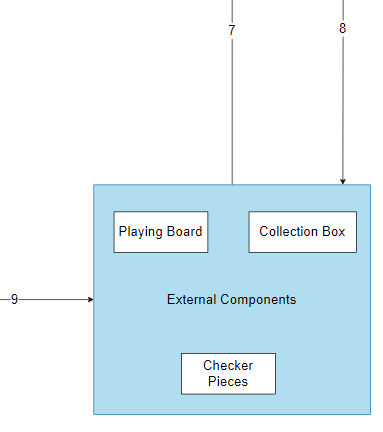
\includegraphics[width=0.60\textwidth]{images/externalComponents_subsystem.png}
 \caption{External components subsystem description diagram}
\end{figure}

\subsection{Playing Board}
% This section should be a general description of a particular subsystem for the given layer. For most subsystems, an extract of the architectural block diagram with data flows is useful. This should consist of the subsystem being described and those subsystems with which it communicates.
The Playing Board is the physical platform with distinct cells which the checkers game is played upon. 

\subsubsection{Assumptions}
% Any assumptions made in the definition of the subsystem should be listed and described. Pay particular attention to assumptions concerning interfaces and interactions with other layers.
Both the robot arm and human opponent interact with the playing board by moving the checkers pieces.

\subsubsection{Responsibilities}
% Each of the responsibilities/features/functions/services of the subsystem as identified in the architectural summary must be expanded to more detailed responsibilities. These responsibilities form the basis for the identification of the finer-grained responsibilities of the layer's internal subsystems. Clearly describe what each subsystem does.
The opponent and the UR5 robot arm will be executing the checkers match upon the playing board. The grid on the playing board sets the boundaries for which movements each player can make. The playing board will be a fixed entity on top of the toolbox and serves as the domain that the camera will be focusing on. 

\subsubsection{Subsystem Interfaces}
% Each of the inputs and outputs for the subsystem are defined here. Create a table with an entry for each labelled interface that connects to this subsystem. For each entry, describe any incoming and outgoing data elements will pass through this interface.

\begin {table}[H]
\caption {Playing Board interfaces} 
\begin{center}
    \begin{tabular}{ | p{1cm} | p{6cm} | p{3cm} | p{3cm} |}
    \hline
    ID & Description & Inputs & Outputs \\ \hline
    \#8 & Camera focuses on the state of the playing board & \pbox{3cm}{N/A} & \pbox{3cm}{State of the playing board}  \\ \hline
    \end{tabular}
\end{center}
\end{table}
%%%%%%%%%%%%%%%%%%%%%%%%%%%%%%%%%%%%%%%%%%%%%%%%%%%%%%%%%%%%%%%%%%%%%%%%%%%%
\subsection{Checkers Pieces}
% Repeat for each subsystem
The checkers pieces are the focus of the two players as they are the items that will be manipulated during the match. 

\subsubsection{Assumptions}
% Any assumptions made in the definition of the subsystem should be listed and described. Pay particular attention to assumptions concerning interfaces and interactions with other layers.
Both the robot arm and human opponent manipulate the checkers pieces by picking up their respective pieces and moving them to a new location.

\subsubsection{Responsibilities}
% Each of the responsibilities/features/functions/services of the subsystem as identified in the architectural summary must be expanded to more detailed responsibilities. These responsibilities form the basis for the identification of the finer-grained responsibilities of the layer's internal subsystems. Clearly describe what each subsystem does.
The checkers pieces are the main objects of the checkers match as both the UR5 arm and opponent will be making decisions on the movement of the pieces. Based on these decisions, both players will be making contact with the checkers pieces in order to manipulate their location. These pieces allow a match to take place.

\subsubsection{Subsystem Interfaces}
% Each of the inputs and outputs for the subsystem are defined here. Create a table with an entry for each labelled interface that connects to this subsystem. For each entry, describe any incoming and outgoing data elements will pass through this interface.

\begin {table}[H]
\caption {Checkers Pieces interfaces} 
\begin{center}
    \begin{tabular}{ | p{1cm} | p{6cm} | p{3cm} | p{3cm} |}
    \hline
    ID & Description & Inputs & Outputs \\ \hline
    \#7 & Opponent manipulates the position of a checkers piece & \pbox{3cm}{Opponent moves a piece} & \pbox{3cm}{New location of the checkers pieces}  \\ \hline
    \#8 & Camera views the pieces on the playing board & \pbox{3cm}{N/A} & \pbox{3cm}{State of a checkers piece}  \\ \hline
    \#9 & UR5 robot arm and magnetic gripper manipulates the position of a checkers piece & \pbox{3cm}{Opponent moves a piece} & \pbox{3cm}{New location of the checkers pieces}  \\ \hline
    \end{tabular}
\end{center}
\end{table}
%%%%%%%%%%%%%%%%%%%%%%%%%%%%%%%%%%%%%%%%%%%%%%%%%%%%%%%%%%%%%%%%%%%%%%%%%%%%
\subsection{Collection Box}
% Repeat for each subsystem
The collection box stands off to the side ready to hold the checkers pieces.
\subsubsection{Assumptions}
% Any assumptions made in the definition of the subsystem should be listed and described. Pay particular attention to assumptions concerning interfaces and interactions with other layers.
The collection box is large enough to carry all checkers pieces and is accessible to both the robot arm and human opponent.

\subsubsection{Responsibilities}
% Each of the responsibilities/features/functions/services of the subsystem as identified in the architectural summary must be expanded to more detailed responsibilities. These responsibilities form the basis for the identification of the finer-grained responsibilities of the layer's internal subsystems. Clearly describe what each subsystem does.
The collection box serves to collect the checkers pieces that are eliminated from the playing board during the checkers match by both the robot arm and human opponent.

\subsubsection{Subsystem Interfaces}
% Each of the inputs and outputs for the subsystem are defined here. Create a table with an entry for each labelled interface that connects to this subsystem. For each entry, describe any incoming and outgoing data elements will pass through this interface.

\begin {table}[H]
\caption {Collection Box interfaces} 
\begin{center}
    \begin{tabular}{ | p{1cm} | p{6cm} | p{3cm} | p{3cm} |}
    \hline
    ID & Description & Inputs & Outputs \\ \hline
    \#7 & Opponent eliminates the robot arm's checkers piece & \pbox{3cm}{Checkers piece disposed into collection box} & \pbox{3cm}{N/A}  \\ \hline
    \#9 & Robot arm eliminates the opponent's checkers piece & \pbox{3cm}{Checkers piece disposed into collection box} & \pbox{3cm}{N/A}  \\ \hline
    \end{tabular}
\end{center}
\end{table}

